\documentclass[a4paper]{article} % A4 paper and 11pt font size

\usepackage{braket}
\usepackage{amsmath}
\usepackage{amssymb}
\usepackage{bm}
\usepackage[utf8]{inputenc}
\usepackage{verbatim}
\usepackage{tikz}
%\usepackage{pgfornament}
\usepackage{pgfplots}
\usepackage{pgffor}
\usepackage[version-1-compatibility]{siunitx}
\usepackage{fancyhdr}
\usepackage{lipsum}
\usepackage{gensymb}
\usepackage{framed}
\usepackage{cancel}
\usepackage{slashed}
\usepackage{hyperref}
\usepackage{pdflscape}
\usepackage{graphicx}
\usepackage{caption}
\usepackage{subcaption}
\usepackage{geometry}
\usepackage{yfonts}
\usepackage{calc}
\usepackage{cite}
\usepackage{siunitx}

\setlength{\parindent}{0em}
\setlength{\parskip}{1em}
\newcommand{\goth}[1]{{\Huge\textfrak{#1}}}
\renewcommand{\baselinestretch}{1.1}

\newcommand{\exercise}[2]
{
\begin{framed}
\textbf{Exercise:} #1 \\\hrule
#2
\end{framed}
}

\newcommand{\example}[2]
{
\begin{framed}
\textbf{Example #1:} #2
\end{framed}
}

\newcommand{\review}[1]
{
\hrule
A short review:

#1
\hrule
}

\renewcommand{\picture}[1]
{
\begin{figure}[h]
\centering
\includegraphics[width=0.5\textwidth]{#1}
\end{figure}
}

\newcommand{\picturesize}[2]
{
\begin{figure}[h]
\centering
\includegraphics[width=#2\textwidth]{#1}
\end{figure}
}

\newcommand{\bmx}[1]{
\begin{bmatrix}
#1
\end{bmatrix}
}

\newcommand{\pmx}[1]{
\begin{pmatrix}
#1
\end{pmatrix}
}

\renewcommand{\tilde}{\widetilde}

 \geometry{
 a4paper,
 total={210mm,297mm},
 left=28mm,
 right=28mm,
 top=30mm,
 bottom=40mm,
 }


%----------------------------------------------------------------------------------------
%	TITLE SECTION
%----------------------------------------------------------------------------------------
%\setlength\parindent{0pt} % Removes all indentation from paragraphs - comment this line for an assignment with lots of text


\pagenumbering{arabic}
\begin{document}
\pagestyle{empty}

\newcommand{\HRule}{\rule{\linewidth}{0.5mm}}

\begin{titlepage}

    \begin{center}
        \textsc{\large SN: 587623}\\[6cm]

        \HRule \\[0.5cm]
		\Huge \textbf{PHYC90012 General Relativity}\\[0.5cm]
        \huge \textbf{Course Summary}\\[0.5cm] 
        \HRule \\[1.5cm]
        \begin{minipage}{0.4\textwidth}
        \begin{center}

        \large By \\[0.75cm]
        \huge Braden \scshape Moore \\[0.5cm]
        \normalsize \normalfont Master of Science \\
        The University of Melbourne \\

        \end{center}
        \end{minipage}

        \vfill

        \large \today
    \end{center}


\newpage
\end{titlepage}
%----------------------------------------------------------------------------------------
\pagestyle{empty}
\tableofcontents
\newpage

\pagestyle{fancy}
\pagenumbering{arabic}
\rfoot{\textsc{Braden Moore, 587623}}
\lfoot{\textsc{\today}}
\lhead{\textsc{Semester 1, 2016}}
\rhead{\textsc{PHYC90012 General Relativity}}
\setcounter{page}{1}
\setcounter{section}{-1}
\section{Syllabus}
\subsection{Part I}
\begin{enumerate}
\item Introduction to gravity
\begin{itemize}
\item Order of magnitude estimates
\item Small amount of quantum gravity
\end{itemize}
\item Equivalence principle + experimental foundations
\item Geometric objects
\begin{itemize}
\item Need to understand geomtric components of GR
\item Vectors, metric, etc. that live on manifolds
\item Laws of nature do not depend on coordinates chosen
\item Hence can write laws of nature in terms of geometric objects w/o reference to coordinates
\end{itemize}
\item Kinematics
\begin{itemize}
\item Time dilation, length contraction in GR framework
\end{itemize}
\item Calculus in curvilinear coordinates
\begin{itemize}
\item Mass and energy curve spacetime
\item Hence geometric objects moved on curved manifolds
\item Distances are not only spatial but temporal; need to use mathematics of small change = calculus
\item Uses the covariant derivative (a geomtetric object; independent of basis/coordinate independent)
\item This point of the course we will not be considering curved space, but instead only curvilinear coords 
\begin{itemize}
\item A flat space can be covered (represented?) by curved coordinates, but an intrinsically curved surface cannot be covered by flat coordinates
\end{itemize}
\end{itemize}
\item Curved spaces
\begin{itemize}
\item Manifolds 
\item How to calculate lengths, volumes, angles in curved spaces
\item Introduces the idea of parallel transport $\Rightarrow$ leads to curvature
\item Define the Riemann tensor, and its children etc. Ricci tensor, ...; these satisfy the Bianchi identities
\end{itemize}
\item Einsten's field equations
\begin{itemize}
\item Stress-energy tensor
\end{itemize}
\item Weak-field limit
\begin{itemize}
\item Gauge transformations
\end{itemize}
\subsection{Part II - Applications}
\item GR phenomena revisited 
\begin{itemize}
\item GPS, Mercury's orbit, gravitational lensing, gravitational redshift, ...
\end{itemize}
\item Gravitational waves
\begin{itemize}
\item Propagation (phase speed, polarisation, ...)
\item Generation*
\item Detection*
\begin{itemize}
\item[*] = together these form the ``antenna problem"
\end{itemize}
\end{itemize}
\item Relativisitic stars
\begin{itemize}
\item neutron stars
\item equation of state (cannot study on Earth because largest nuclei only have 200 elements or so; need more density)
\end{itemize}
\item Black holes
\begin{itemize}
\item Event horizons, singularities, ...
\end{itemize}
\item Cosmology
\begin{itemize}
\item Friedman-Robertson-Walker (FRW) metric - describes a homogeneous, isotropic universe
\begin{itemize}
\item We will derive this and the Friedman equations
\end{itemize}
\end{itemize}

\end{enumerate}


\section{Introduction to gravity}
\subsection{Strength of gravity}
\begin{itemize}
\item Weak! Weakest of all fundamental forces
\item Long-ranged force (like EM)
\item Weakness determined by coupling constant
\item Coupling constant = Newton's gravitational constant
\end{itemize}
\begin{equation}
\vec{F}=\frac{Gm_1 m_2}{r_{12}^2}\hat{r}
\end{equation}
\begin{itemize}
\item G is hard to measure; least well known of coupling constants
\end{itemize}
In 1797-98, Cavendish used torsion balls (1.8m torsion balance) with rod of big masses and rod of small masses. 
\begin{itemize}
\item Spring constant of torsion balance was measured from free oscillation
\item then introduced 158kg balls
\item measured deflection angle of balance $\Rightarrow$ can calculate force
\begin{itemize}
\item using a mini-telescope against Vernier scale
\end{itemize}
\item rearrange Newton's law to get G
\end{itemize}

\picture{images/cavendish-torsion-balance.png}
 
\exercise{Show that Cavendish also measured density of Earth as a bonus at the same time.}
{Mass of Earth $M_{\oplus}= \rho V$ where $V=\frac{4}{3}\pi R^3$ assuming the Earth is a sphere. How does calculating $G$ also calculate $\rho$? Well, we have $\vec{F}=\frac{Gm_1 m_2}{r_{12}^2}\hat{r}$. Let's take $m_1 = M_\oplus$ as the mass of the Earth, and $m_2 = m$ as some small object mass. Let's imagine the smaller object falling to the center of the Earth. We'll take $r_{12}$ as the distance from the object to the Earth's center, which we can approximate as Earth's radius, i.e. $r_{12}=R$. This force should be equivalent to $F=ma$.\\
\\
So we have
\begin{align*}
\frac{GM_\oplus m}{R^2}&=mg\\
\frac{G\rho \frac{4}{3}\pi R^3}{R^2}&=g\\
\frac{4G \rho \pi R}{3}&=g\\
\Rightarrow \rho &=\frac{3g}{4\pi GR}\\
&=\frac{3\times \SI{9.8}{ms^{-2}}}{4\pi\times \SI{6.67384d-11}{\kg^{-1}\m^3 \s^{-2}}\times \SI{6370}{km}}\\
&=\frac{3\times 9.8}{4\pi\times 6.67384\times 10^{-11}\times 6370\times 10^3}\si{\kg.m^{-3}}\\
&=\SI{5503}{kg.m^{-3}}
\end{align*}
}


\begin{itemize}
\item Modern $G=6.67384(80)\times \SI{d-11}{Nm^{-2}.\kg^{-2}}=\si{\kg^{-1}.\m^3.\s^{-2}}$
\item Product GM is known to 1 part in $\sim 10^{10}$ from astrophysics observations
\begin{itemize}
\item[$\Rightarrow$] mass is hard to measure gravitationally
\end{itemize}
\item We need a dimensionless number to characterise strength
\item Newton: $\Phi=\frac{GM}{r}$ (potential)
\item In free fall: $\frac{KE}{mass}$, $v^2 \sim \frac{GM}{r}$
\item We claim gravity is strong is free-fall is relativistic, i.e. $v\sim c$
\item This is an order of magnitude estimate
\end{itemize}


\subsection{Strong vs. weak gravity}
\begin{itemize}
\item Quasi-Newtonian:
\begin{itemize}
\item characterticstic speed of body in free fall: $v^2\sim \frac{GM}{r}$
\end{itemize}
\item Strong gravity leads to relativistic free fall, i.e. $\frac{GM}{Rc^2}\geq 1$ where M is the total mass and R is th characteristic size
\end{itemize}

\begin{table}
\centering
\begin{tabular}{c|cc} 
 & $\frac{GM}{Rc^2} \lll 1$ & $\frac{GM}{Rc^2}\geq 1$\\
\hline $v \ll c$ & Newtonian & CAN'T EXIST \\
$v\sim c$ & special rel. & full GR (difficult)
\end{tabular}
\end{table}

\example{1.1}{
$M=M_{\odot}$ (mass of the Sun)
\begin{align*}
R & \sim \frac{GM}{c^2} \text{\quad boundary of strong regime}\\
&\sim \frac{10^{-10}10^{30}}{10^{17}}\\
&\sim \text{km}
\end{align*}
cf. Schwarz radius of black hole $=\frac{2GM}{c^2}$
}
\example{1.2}{
Density of black hole with mass of $M_\odot$
\begin{align*}
&\sim \frac{M}{R^3}\sim\frac{\SI{d30}{kg}}{\si{(km)^3}}\\
&\sim 10^{21}kgm^{-3}
\end{align*}
How does this density compare to maximum density of (say) nuclear matter? Let's compare.
\begin{align*}
\frac{m_n}{(1fm)^3}\sim \frac{10^{-27}kg}{10^{-45}m^3}\sim 10^{18}kgm^{-3}
\end{align*}
We see a black hole is more dense that a nuclei. The characteristic size of a particle $1fm\sim\Delta x\sim \frac{\hbar}{\Delta p}\sim \frac{\hbar}{m_n c}$, due to Heisenberg's uncertainty principle, and also the Pauli exclusion principle.
}
More generally: density of material that froms black hole $\sim\frac{M}{R^3}$, but note $M=\frac{c^2R}{G}$ density $\rho \propto \frac{1}{R^2}$. This means that denser black holes are smaller.

\exercise{Estimate the strength of gravity $\frac{GM}{Rc^2}$ on Earth.}

\example{2}
{
The Universe is composed of 5\% baryons + 25\% dark matter + 70\% dark energy. Estimate M and R.\\\hrule
$R\sim \SI{10}{Gpc}$
\begin{itemize}
\item Mass of baryons 
\begin{itemize}
\item $10^{11}$ stars in Milky Way
\item $(10^4)^3$ galaxies in Universe
\item[$\Rightarrow$] $M_{\text{baryons}}\sim10^{23}M_\odot\sim \SI{d53}{kg}$
\end{itemize}
\end{itemize} 
\begin{equation}
\frac{GM_{tot}}{Rc^2}\sim\frac{10^{-10}\cdot 10^{53}\cdot 10}{10^{27} \cdot 10^{17}}\sim 1
\end{equation}
\begin{align*}
\text{Density }\rho\sim\frac{M_{tot}}{R_{tot}^3}&\sim\frac{c^2}{R^2G}\text{, use }\frac{GM}{Rc^2}\sim 1\\
&\sim\frac{1}{G\times(\text{age of universe})^2}
\end{align*}
cf. critical density from Friedmann equations $\rho_{crit}=\frac{3H_0^2}{8\pi G}$.\\
Recall Hubble constant $H_0\sim \frac{1}{\text{age}}$.
}
The critical density is the density of the universe at which expansion will asymptotically slow. Too dense leads to big crunch, too low leads to unbounded expansion.
\exercise{How do we reconcile a ``flat" universe from critical density with the ``curved" universe?}

Important to remember: gravity is strong when $\frac{GM}{Rc^2}\sim 1$, which occurs around black holes, the universe at large. In a sense, cosmological results such as critical density, expansion of universe come from this.

\subsection{Black hole oscillations}
We can estimate the oscillation frequency of a ``black hole'' (i.e. something with $\frac{GM}{Rc^2}\sim 1$ as $\sim \frac{c}{R}$; that is, the time is takes light to travel the distance of the object. This is the natural frequency for this object. Using that ubioquitous expression we can express the oscillation frequency as $\sim \frac{c^3}{GM}$, e.g. $M=M_\odot \Rightarrow \text{frequency}\sim\SI{10}{kHz}$.

Let's discuss charged black holes. It is difficult to astrophysically have charged black holes, because stars are not usually charged (due to the strength of the EM force, which would attract opposite charge and cancel out). So, these are artificial in nature. These have unusual geometry, and are called ``Reissner-Nordstrom'' black holes.
\example{}{What is the maximum charge on a black hole?\\\hrule
\begin{align*}
\frac{Q^2}{4\pi\epsilon_0 R}&\leq \frac{GM^2}{R}\\
Q&\leq (4\pi\epsilon_0 G)^{1/2} M
\end{align*}
Above, we relate Coloumb force to gravitational force. The gravitational force holding a black hole together must overcome the Coloumb force pushing it apart.
}

\subsection{Quantum Gravity}
The problem wtih quantum gravity is that there is no theory... hence we must rely on numerology.

We consider a hypothetical elementry excitation of a ``black hole'' (again, we mean a \emph{relativistic compact object}) of mass $M$. Hence the characteristic size, or ``wavelength'', of the excitation is $\frac{GM}{c^2}$ (fundamental excitation only). Introducing quantum mechanics: the Heisenberg uncertainty principle tells us that the zero-point motion associated with this excitation is
\begin{equation}
\lambda\sim\frac{\hbar}{\Delta p}\sim \underbrace{\frac{\hbar}{Mc}}_{\text{relativisitic}}
\end{equation}
Equating length scales $\Rightarrow M_{pl}\approx \left(\frac{\hbar c}{G}\right)^{1/2}$; this is the Planck mass, about $\SI{d-8}{kg}$ (the mass below which quantum gravity is important. 

Given $M_{pl}$ we get $\lambda\sim\frac{\hbar}{M_{pl}c}\sim \SI{d-33}{m}$; the Planck length - the length where quantum gravity is important (e.g. just after Big Bang).

\subsubsection{Hawking Radiation}
Let's return to our elementary excittion with $\lambda\sim\frac{GM}{c^2}$, i.e. frequency $\sim \frac{c^3}{GM}=\frac{c}{\lambda}$. Heisenberg tells us there is an associated energy fluctation $\Delta E\sim h\times\text{frequency}\sim\frac{\hbar c^3}{GM}$. Suppose (note: this is a huge leap) energy fluctuation in the black hole sysytem is in thermal equilibrium with a bath at temperature $T$. Then $T\sim\frac{\Delta E}{k_B}$. This associates a temperature to a black hole.

We call a black hole a blackbody! 
\begin{align*}
\text{Radiated power }&= k_B\times \text{area} \times T^4\\
&=\sigma\times \underbrace{R^2}_{\left(\frac{GM}{c^2}\right)^2}\times \left(\frac{\hbar c^3}{GMk_b}\right)^4\\
&\propto M^{-2}
\end{align*}

\exercise{Plug in numbers to this!}{}

This shows that a black hole radiates energy $\Rightarrow$ eventually a black hole evaporates. We can estimate the time scale of this evaporation.
\begin{equation}
\text{time scale}\sim\frac{Mc^2}{\text{power}}\propto M^3
\end{equation}
$\Rightarrow$ small black holes evaporate fast!

As an aside, we could consider the rate of energy accretion. For system outside a black hole with uniform density $\rho_{\text{out}}$, we have
\begin{align*}
\text{rate of mass accretion}&\sim \rho_\text{out}\cdot c \cdot 4\pi R^2\\
\text{rate of energy accretion}&\sim c^2\cdot \text{rate of mass accretion}
\end{align*}
\hrule
A short review:
\begin{itemize}
\item there is no theory of quantum gravity
\item we consider a relativisitic elementary oscillation $\lambda\sim\frac{GM}{c^2}$
\item we use Heisenberg to relate this to an enegy fluctutation in the system
\item energy fluctuation can be converted to a temperature $T_H=\frac{\hbar c^3}{GMk_B}$, the Hawking temperature
\item we find small block holes evaportate more quickly than large black holes
\end{itemize}

\hrule

\subsection{Black hole thermodynamics}
\textbf{1st law}: $dS=\frac{dQ}{T}$\quad system constant volume

Hawking radiation: we lose a bit of heat $dQ$ due to blackbody radiation.
\begin{equation}
dS=\frac{GMk_b}{\hbar c^3} d(Mc^2)
\end{equation}
We see heat loss comes from rest energy
\begin{equation}
\frac{dS}{k_B}\approx \frac{1}{R^2_{\text{Planck}}}\underbrace{d(R^2)}_{R\sim\frac{GM}{c^2}}
\end{equation}
This result relates the entropy of a black hole to its area; Bekenstein-Hawking entropy - $S_{\text{black hole}}\propto\text{area of event horizon}$.
\begin{equation}
\frac{S}{k_B}=\frac{\text{area}}{4R^2_{\text{Planck}}}\footnote{In 1995, Maldacena also got this by counting microstates}
\end{equation}

However, there is a contradiction! Hawking radiation implies that $dA<0 \Rightarrow dS<0$.... this is bad.\footnote{See Ted Jacobson's lecture at University of Utrecht for a discussion on this.} One way to resolve this is by makung a generalised \textbf{2nd law}:
\begin{equation}
d\left(S_{\text{outside}}+\frac{\text{area}}{4R_{\text{Planck}}^2}\right)\geq 0
\end{equation}
Unfortunately this is not enough - there is still a contradiction. Consider a small box of radiation which we prepare far from a black hole. $S_{\text{box}}=\frac{4U_{\text{box}}}{3T_\text{box}}$. We can make photons very long wavelength, so that $U_{\text{box}}\approx 0$ byt $S_{\text{box}}\neq 0$. Then $dS_{\text{out}}=-S_{\text{box}}<0$. $d(\text{area})=0$ because energy in box $=0$, i.e. $d(Mc^2)=0$.\footnote{Beware the Unruh radiation.}

\exercise{Resolve the box paradox!}{}

\textbf{3rd law of BH thermodynamics}: can't reduce $T$ to zero.\footnote{If you are curious: Verlinde, 
\href{arXiv.org/abs/1001.0785}{arXiv:1001.0785}, \emph{On the Origin of Gravity and the Laws of Newton}, in which the idea of emph{gravity is an entropic force} is discussed.}

In heating a rubber band, it shrinks; this is because a shrunken arrangement of the molecules is a state of more entropy (more disordered)

\begin{center}
{
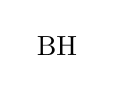
\begin{tikzpicture}
\node at (0,0) {BH};
\end{tikzpicture}
}
\end{center}

																					
\section{Einstein equivalence principle}
We will define this (the weak and strong equivalence principles), and some of the tests been performed.

\subsection{Weak equivalence principle}
Trajectory of body in free fall is independent of its mass and $\underbrace{\text{composition}}_{\text{binding energy}}$ (as per Galileo, feather vs. brick). Note that this is not equivalent for electric fields (the movement of a charged particle through an electric field depends on its charge).

\subsection{Strong equivalence principle}
\begin{enumerate}
\item weak equivalence principle is valid
\item results of any non-gravitational (e.g. EM, \underline{not} Cavendish expt) experiment is independent of velocity fo freely falling frame
\begin{itemize}
\item this is \emph{local lorentz invariance}
\end{itemize}
\item results of non-gravitational experimental are indepent of where and when it is performed
\begin{itemize}
\item this is \emph{local position invariance}
\end{itemize}
\end{enumerate}

The Einstein equivalence principle (EEP) $\equiv$ strong implies: existence of a ``curved spacetime'' with:
\begin{enumerate}
\item[\textbf{i.}] symmetric metric
\item[\textbf{ii}.] trajectories of free-falling bodies are geodesicas of metric
\item[\textbf{iii.}] the laws of physics in a freely-falling frame can be written in the lnaguage of special relativity
\end{enumerate}


\review{
Einstein equivalence principle:
\begin{enumerate}
\item universality of free fall
\item local Lorentz invariance
\item local position invariance
\end{enumerate}
Implications:
\begin{enumerate}
\item[3)] $\Rightarrow$ fundamental constant independent of $\vec{x}$, $t$
\item[2)] $\Rightarrow$ laws of non-gravitational physics \underline{locally} independent of frame
\item[1)] $\Rightarrow$ space is \underline{curved}
\end{enumerate}

Why is space curved? Locally straight trajectory in free yet \underline{yet} gravity producess curved trajectory (observed) $\Rightarrow$ only possible if coordinates change from one point to next
}

\section{Experimental tests}
\subsection{Experimental tests of free fall}
Inertial mass $m_i=\frac{\text{applied non-gravitational force}}{\text{measured acceleration}}$

Gravitational mass $m_g=$ ``passive'' mass appearing in weight

Look for $m_i \neq m_g$

Write 
\begin{equation}
m_g=m_i + \sum_{\text{interactions A in body}}\eta^A \frac{E^A}{c^2}
\end{equation} 
Here $E=$ ``binding energy''/potential energy of interaction $A$.

\underline{Tests:}
\begin{enumerate}
\item E{\"o}tv{\"o}s-type torsion balance experiements: two different materials may fall at difference rates (see Dicke, Braginsky)
\item Colorado: U, Cu laser interferometer $\Rightarrow relativite acceleration$
\item E{\"o}t-Wash experiements: fancy version of 1)
\end{enumerate}

Result:
\begin{equation}
\frac{|m_g-m_i|}{m_i}\leq 10^{-13}
\end{equation}

We test this, for eample, with aluminium (Al) and gold (Au) weights on a torsion balance. As the Sun moves from one side of the Earth to the other, if the gravitational mass of either differs from the other we will see diurnal oscillation in the balance.

\picture{images/eotvos.png}

\subsection{Tests of local Lorentz invariance}
\begin{itemize}
\item Michelson-Morley experiment (the aether)
\item Rossi-Hall tests for lifetime of muons (time dilation $\Leftrightarrow$ LLI)
\item Ives-Stiwell transverse Doppler shift
\begin{itemize}
\item laser travelling some vector $\vec{v}$
\item we see perpendicular wave vector $\vec{k}$
\item measure frequency when laser intersects line of sight
\item Doppler shift arises due to time dilation
\end{itemize}
\end{itemize}

Mathematically:
\begin{equation}
\bmx{\omega'/c\\k'_x\\k'_y\\k'_z}=
\bmx{
\gamma&\gamma v/c&0&0\\
\gamma v/c&\gamma&0&0\\
0&0&1&0\\
0&0&0&1
}
\bmx{
\omega/c\\0\\k_y\\0
}=
\bmx{
\gamma\omega/c\\
\gamma\omega v^2/c\\
k_y\\
0
}
\end{equation}

\exercise{Compare with standard longitudinal Doppler:
\begin{equation}
\pmx{\\\text{same}\\\text{matrix}\\\\}\pmx{\omega/c\\k_x\\0\\0}
\end{equation}
}
{}

\review{Last lecture:
\begin{itemize}
\item tests of LPI
\item Schiff's thought experiement (gravitational redshift)
\end{itemize}
}

\subsection{Gravitational redshift}
\begin{equation}
\frac{h\nu'-h\nu}{h\nu}=\frac{(m_A g_A - m_B g_B)H}{(m_A-m_B)c^2}
\end{equation}
If $g_A=g_B$ (universal free-fall), then gravitational redshift is $gH/c^2$

\subsection{Observation of GR in experiments}
There are situtations where GR makes measurable difference \underline{today}

\begin{itemize}
\item Pound-Rebka experiment (gravitational redshift, also seen on white dwarf spectral lines)
\item GPS
\item 2015 discovery of gravitational waves from binary BH merger
\item cosmological measurements (CMB, redshifts, $H_0$, \ldots)
\item gravitational lensing (light bent by a mass) (see: Einstein cross, Abell clusters, stars behind Sun)
\item precession of perihelion of Mercury
\item orbital decay of Hulse-Taylor binary pulsar (can calculate to mm precision the decay of the orbit every 8 hours due to gravitational wave emission)
\item Nordtredt/lunar ranging experiments
\item Gravity Probe B - lense-thinning precession
\item Shapiro time delay
\end{itemize}

\begin{figure}[h]
\centering
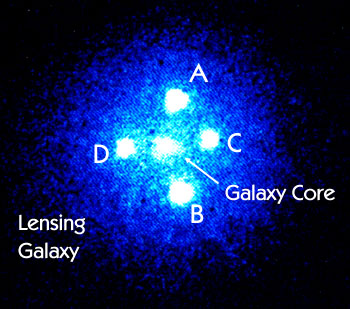
\includegraphics[width=0.5\textwidth]{images/einstein-cross.jpg}
\caption{Einstein cross}
\end{figure}


\subsubsection{Pound-Rebka experiment}
Looks at gravitational redshift of $\SI{14.4}{keV}$ gamma rays from $^{57}$Fe decay

$^{57}$Fe decays and emits photons directly down from a $\SI{23}{m}$ tall tower, to another box of $^{57}$Fe below. Gravitational redshift occurs; time moves slower closer to the Earth, so gamma ray emitted will have a different energy than that required to be absorbed by the $^{57}$Fe at the bottom.

Receiver box moves up/down at speed $v$. We adjust $v$ at bottom so that kinematic Doppler shift $\propto \left(\frac{1-v/c}{1+v/c}\right)^{1/2}$ exactly cancels the gravitational redshift $\propto gH/c^2$

N.B.: recoil (in a random direction) when photon emitted/absorbed; energy $E_R=\frac{E_\gamma}{2M_{Fe}c^2}$

\begin{equation}
E_R\sim\frac{\SI{14.4}{keV}}{\SI{100}{GeV}}\sim 10^{-7}
\end{equation}

We solve this problem through the Mossbauer effect: use whole crystal; whole crystal ($\sim10^{23}$ Fe atoms) recoils

\begin{figure}[h]
\centering
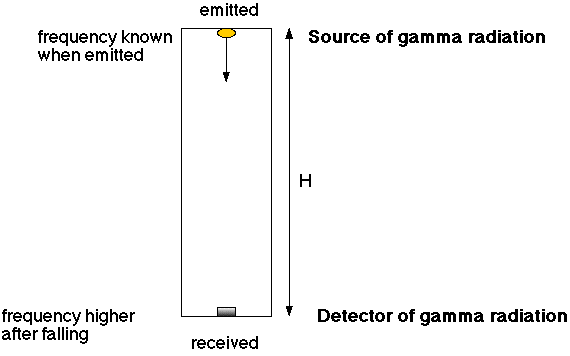
\includegraphics[width=0.5\textwidth]{images/pound-rebka.png}
\caption{Pound-Rebka experiment}
\end{figure}


\subsubsection{Lunar ranging}
Williams + Dickey (2002)\footnote{See also ``Living Reviews'' Relativity}

Moon not completely dormant
\begin{itemize}
\item fluid core (?)
\item tidal dissipation internally
\item etc \ldots
\end{itemize}

Multiple radar reflectors to improve accuracy. We search for an accurate Earth-Moon orbit versus time; we find
\begin{equation}
\frac{1}{G}\frac{dG}{dt}=(0.0\pm 1.1)\times \SI{d-12}{yr^{-1}}
\end{equation}

Uncertainty $\approx 0.02 H_0$ - we don't see increasing separation between Earth and Moon due to expansion of universe. This is expected, however: gravitational bound objects do not separate with time, although the energy they require to stay bound will increase

\subsubsection{Deflection of light (gravitational lensing)}
In a three-body system with the Earth, the Sun and another star, the light from the star will bend due to the Sun before it reaches Earth (not taking a straight path). This causes the apparent position of the star to be different than the actual position.

Deflection angle $\delta\theta \propto \frac{GM}{c^2d}$

GR deflection = $2\times$ Newtonian deflection (Einstein 1911). 

This effect is achromatic!

\subsubsection{Shapiro delay}
Roundtrip time from Earth to a distant mirror (in a three-body system including the Sun) is longer than if the Sun was not there.
\begin{equation}
\delta t\propto \frac{GM}{c^3}\ln(\text{geometric factors})
\end{equation}

Best measurements with Cassinin spacecraft (accuracy 1 in $10^5$)

\section{Geometric Objects}

\subsection{Vectors}
Invariants are measurable. Therefore, each coordinate represenation is as valid as the other!

\subsubsection{Definitions of a vector}
Vector $\vec{A}$
\begin{itemize}
\item four numbers that are projections onto spacetime (can be dependent or indepedent of a metric)
\begin{itemize}
\item Note: vectors can have meaning without a metric
\end{itemize}
\item a geometric object with ``length'' (requires a metric) and a ``direction'', i.e. an arrow
\item a geometric object which transforms from one coordinate system to another
\item a linear function which trakes a 1-form as an argument and returns a real numver
\end{itemize}

$\underbrace{\text{Vector spaces}}_{\text{vectors}}\supseteq \underbrace{\text{normed vector spaces}}_{\text{length}} \supseteq \underbrace{\text{inner product spaces}}_{\text{angle}}$

$\Rightarrow$ you can have vector spaces wirthout a norm or angle concept.

\exercise{$\vec{\Delta}x=$ displacement (in spacetime), is a vector}{}

Vector components, $A^0,A^1,A^2,A^3$; in another frame we have $A^{0'},A^{1'},A^{2'},A^{3'}$.

\subsubsection{What is a basis vector?}
Projection requires a metric (for a dot product)!
$\Rightarrow$ we have 4, special, linearly independent vectors which ``point along'' (no concept of length/angle) axes of coordinate system, $\left\{\vec{e}_{\alpha}\right\}$

\begin{equation}
\vec{A}=A^0 \vec{e}_{0} +A^{1}\vec{e}_{1}+A^{2}\vec{e}_{2}+A^{3}\vec{e}_{3} \label{vector projection}
\end{equation}

As $\vec{e}_{0}$ is itself a vector, using \ref{vector projection}
\begin{equation}
\vec{e}_{0}=(\vec{e}_{0})^{0}\vec{e}_{0}+(\vec{e}_{0})^{1}\vec{e}_{1}+(\vec{e}_{0})^{2}\vec{e}_{2}
+\underbrace{(\vec{e}_{0})^{3}}_{\text{3rd component of }\vec{e}_{0}}\vec{e}_{3}
\end{equation}

By linear independence, as $\vec{e}_0$ is linearly independent to $\vec{e}_{1},\vec{e}_{2},\vec{e}_{3}$
\begin{equation}
\Rightarrow (\vec{e}_{0})^{1}=(\vec{e}_{0})^{2}=(\vec{e}_{0})^{3}=0
\end{equation}
\begin{equation}
\Rightarrow (\vec{e}_{\alpha})^{\beta}=\delta_{\alpha}^{\beta}
\end{equation}
which is \emph{true in all coordinate systems}. Therefore in a primed frame,
\begin{equation}
\Rightarrow (\vec{e}_{\alpha'})^{\beta'}=\delta_{\alpha'}^{\beta'}
\end{equation}

\underline{But} $(\vec{e}_{\alpha'})^{\beta}\neq \delta^{\beta}_{\alpha'}$
\begin{itemize}
\item $\vec{e}_{\alpha'}$ is tied to the prime frame
\item the geometric object is only defined with respect to the frame (where $\vec{A}$ could exist in all frames)
\item you cannot measure a basis vector in another coordinate frame. You have to be in the coordinate frame to measure it.
\end{itemize}

\subsubsection{Transformations}
In general,
\begin{align*}
\left\{x^{\beta'}\right\}&\mapsto \left\{x^{\alpha}\right\}\\
from \sigma' &\to \sigma\quad\text{primed to unprimed}
\end{align*}

\begin{equation}
\Lambda^{\alpha}_{\beta'}=\frac{\partial (x^{0},x^{1},x^{2},x^{3})}{\partial (x^{0'},x^{1'},x^{2'},x^{3'})}
=\frac{\partial x^{\alpha}}{x^{\beta'}}\quad \text{16 elements!}
\end{equation}

If the transform is linear (e.g. Lorentz transform), we can consider
\begin{equation}
x^{\alpha}=\Lambda^{\alpha}_{\beta'}x^{\beta'}
\end{equation}
where $\Lambda^{\alpha}$ is not necessarily a constant. But if the transform is non-linear, the left side is wrong. We instead have
\begin{equation}
dx^{\alpha}=\Lambda^{\alpha}_{\beta'}~dx^{\beta'}
\end{equation}

Why? If we define $\vec{x}$ as a displacement from origin to the point in a curved space, there are mutliple different path. We would need more than 4 numvers to define this, therefor we no longer have a meaningful vector. 

Vectors are defined localling an tangent space, \textbf{and} transformations of vectors are also restricted locally to trangent space. If $\vec{A}$ is a vector,
\begin{equation}
A^{\alpha}=\Lambda^{\alpha}_{\beta'}A^{\beta'}
\end{equation}

\review{\textbf{Vectors}

$\vec{A}$: defined in tangent space

Components $A^\alpha$: $\vec{A}=A^\alpha \vec{e}_{\alpha}$ where $\vec{e}_{\alpha}$ are basis vectors. These (unprimed) basis vectors only have meaning in unprimed coordinates

Transform like infinitesimal displacements:
\begin{equation}
\underbrace{A^{\alpha'}}_{\text{primed}}=\overbrace{\frac{\partial x^{\alpha'}}{\partial x^{\alpha}}}^{\text{transform matrix}}\underbrace{A^{\alpha}}_{\text{unprimed}}\label{vector transform}
\end{equation}

How do basis vectors transform?
\begin{align*}
A^{\alpha}\vec{e}_\alpha=\vec{A}&=A^{\alpha'}\vec{e}_{\alpha'}\\
&=\frac{\partial x^{\alpha'}}{\partial x^{\beta}}A^{\beta}\vec{e}_{\alpha'}	\\
&=\frac{\partial x^{\alpha'}}{\partial x^{\alpha}}A^{\alpha}\vec{e}_{\alpha'}
\end{align*}

This has to be true for all $\vec{A}$, i.e.
\begin{equation}
\vec{e}_{\alpha}=\frac{\partial x^{\alpha'}}{\partial x^{\alpha}}\vec{e}_{\alpha'}
\end{equation}
Or equivalently,
\begin{equation}
\vec{e}_{\alpha'}=\frac{\partial x^{\alpha}}{\partial x^{\alpha'}}\vec{e}_{\alpha}
\end{equation}
Note this is the opposite of transformation law for vector components \ref{vector transform}

\exercise{Try for Lorentz transformations.}{}
\exercise{(later) Try for 2 types of Schwarz black hole coordinates.}{}

}

\subsection{1-forms}
$\widetilde{p}$
\begin{itemize}
\item four numbers assocation to four dimensions and associated to vectors in a specific way (see below)
\item geomtric objecs that transforms like a \underline{gradient}
\item tensor of type $\pmx{0\\1}$, i.e. linear function which accepts vector as an argument and reutrns a real number
\end{itemize}
If we have a metric, a neat way to visualise a 1-form is as a contour.

e.g. vector is an arrow (length, direction)

cf. 1-form is contours

\picturesize{images/contour.png}{0.3}
Value of $\widetilde{p}(\vec{A})=4$; number of times $\vec{A}$ pierces surfaces of $\widetilde{p}$

Components defined to be
\begin{align*}
p_\alpha&=\widetilde{p}(\vec{e}_{\alpha})\\
&=\langle{\tilde{p},\vec{e}_{\alpha}}\rangle
\end{align*}
From lines 1 to 2, we have equivalent notation. We are using an inner product. By convention we use a lowered index.

We cannot have curved contours, as they are only defined in tangent space.

We have a neat way to calculate the coordinate-independent quantity $\tilde{p}(\vec{A})$
\begin{align*}
\tilde{p}(\vec{A})&=\tilde{p}(A^{\alpha}\vec{e}_{\alpha})\\
&=A^{\alpha}\tilde{p}(\vec{e}_{\alpha})\quad\text{linear}\\
&=A^{\alpha}p_{\alpha}
\end{align*}

This is a contraction. It is an inner product but \underline{not} dot product (we require a metric, and for it to be between two vectors, for a dot product).

Vectors and 1-forms are ``apples and oranges'' - completely different geometric objects which cannot be compared even at the same point, e.g. $\tilde{p}=\vec{A}$ is meaningless.

This is comparable to bras and kets in quantum mechanics; they form a dual space, but we cannot directly compare the objects of a pair

\subsubsection{How do 1-forms transform?}
We start with basis vectors
\begin{equation}
\vec{e}_{\alpha}=\frac{\partial x^{\alpha'}}{\partial x^{\alpha}}\vec{e}_{\alpha'}
\end{equation}
In component form:
\begin{align*}
p_{\alpha'}&=\tilde{p}(\vec{e}_{\alpha'})\\
&=\frac{\partial x^{\alpha}}{\partial x^{\alpha'}}\tilde{p}(\vec{e}_{\alpha})\quad\text{linear}\\
&=\frac{\partial x^{\alpha}}{\partial x^{\alpha'}}p_{\alpha}
\end{align*}
i.e. components of $\tilde{p}$ transform like basis vectors (\underline{not} components of basis vectors)


\pagebreak

%-----------------------------------------
\end{document}




%\begin{tikzpicture}[line width=0.7 pt, xscale = 3, yscale = 3]

%\draw [fermion] (0,0)--(1.5,0);
%	\node at (0.75,0.3) {$\tau$};

%\end{tikzpicture}



